% !TEX encoding = UTF-8
% !TEX TS-program = pdflatex
% !TEX root = computabilità e algoritmi.tex
% !TEX spellcheck = it-IT
\section{I primi problemi semplici:}\label{la-soluzione-ai-semplici-problemi}



\begin{itemize}
	\item
	Dati due segmenti orientati con un vertice in comune, il secondo segmento è ruotato in senso orario o antiorario rispetto il primo?
	\item
	Seguendo il percorso dato da due segmenti orientati, per spostarmi sul secondo devo girare a sinistra o a destra?
	\item
	Due segmenti si intersecano?
\end{itemize}

Abbiamo però il limite che non possiamo utilizzare la divisione e le funzioni trigonometriche perché abbiamo a disposizione solo numeri interi.


\subsection{Rotazione in senso orario o antiorario}\label{rotazione-in-senso-orario-o-antiorario}

In questo caso basta calcolare il prodotto vettoriale

\begin{breakablealgorithm}
	\caption{\textsc{Angle-Left}: angolazione di un segmento rispetto ad un segmento di riferimento}
	\begin{algorithmic}[1]
		\Function{Angle-Left}{$p_0,p_1,p_2$}
			\State $d = (x_1-x_0)(y_2-y_0) - (x_2-x_0)(y_1-y_0)$
			\State \Return $d$
		\EndFunction
	\end{algorithmic}
\end{breakablealgorithm}

\emph{d} risulta essere maggiore di 0 se l'angolo tra i segmenti $\overrightarrow{p_0p_1}$ e $\overrightarrow{p_0p_2}$ è orientato in senso antiorario, se invece è minore di 0 l'angolo è
ruotato in senso orario e se è uguale a 0 l'angolo è 0 oppure uno dei
due segmenti è degenere.

\subsection{Il giro del volante}\label{il-giro-del-volante}

Devo girare a sinistra se tra $\overrightarrow{p_0p_1}$ e il vettore $\overrightarrow{p_0p_2}$ c'è una rotazione in senso antioraria. (Da notare che in questo caso i segmenti di interesse sono $\overrightarrow{p_0p_1}$ e $\overrightarrow{p_1p_2}$).

\begin{breakablealgorithm}
	\caption{\textsc{Turn-Left}: rotazione rispetto ad un segmento}
	\begin{algorithmic}[1]
		\Function{Turn-Left}{$p_0,p_1,p_2$}
			\State $d \gets \textsc{AngleLeft}(p_0,p_1,p_2)$
			\State \Return $d$
		\EndFunction
	\end{algorithmic}
\end{breakablealgorithm}

Se $d >0 $ c'è una svolta a sinistra, se invece è minore di 0 la svolta è a destra e se è 0 si prosegue nella stessa direzione o si fa un'inversione ad U.

\subsection{Intersezione di due segmenti}\label{intersezione-di-due-segmenti}

Si vuole sapere se i due segmenti $\overline{p_1p_2}$ e $\overline{p_3p_4}$ si intersecano o meno.

Ci sono due possibili casi:

\begin{enumerate}
\item
  I due segmenti stanno sulla stessa retta (collineari). In questo caso si intersecano solo se uno dei due estremi $p_3$ o $p_4$ appartiene al segmento $\overline{p_1p_2}$ oppure uno dei due segmenti contiene l'altro.
\item
  I due segmenti non sono sulla stessa retta. In questo caso bisogna vedere se $p_1$ e $p_2$ stanno dalla parte opposta della retta $\overline{p_3p_4}$ e se $p_3$  e $p_4$ stanno dalla parte opposta della retta $\overline{p_1p_2}$.
\end{enumerate}

Per verificare che due segmenti siano collineari basta calcolare il prodotto vettoriale

$$
d_1 = (p_1-p_3) \times (p_4-p_3) \text{// } p_1\text{ rispetto } \overline{p_3p_4}
$$

Se uno dei due segmenti è degenere si ottiene sempre $d_1 = 0$, è necessario quindi verificare che non ci siano segmenti degeneri.

\begin{align*}
d_2 &= (p_2-p_3) \times (p_4-p_3) \text{// } p_2\text{ rispetto } \overline{p_3p_4}\\
d_3 &= (p_3-p_1) \times (p_2-p_1) \text{// } p_3\text{ rispetto } \overline{p_1p_2} \\
d_4 &= (p_4-p_1) \times (p_2-p_1) \text{// } p_4\text{ rispetto } \overline{p_1p_2}
\end{align*}

Se $d_1 = d_2 = 0$ o i due segmenti sono sulla stessa retta o $\overline{p_3p_4}$ è degenere. 
Se $d_3=d_4=0$ o i due segmenti sono sulla stessa retta o $\overline{p_1p_2}$ è degenere.

Basta quindi calcolare i 4 prodotti scalari e controllare se sono tutti 0. In caso affermativo si ha che i due segmenti sono collineari ed è corretto anche se entrambi i segmenti sono degeneri perché due segmenti degeneri sono anche collineari. Per verificare se i due segmenti si intersecano basta quindi controllare se $p_3$ o $p_4$ sono interni da $\overline{p_1p_2}$ oppure se $\overline{p_1p_2}$ è interno a $\overline{p_3p_4}$.

Se almeno uno dei prodotti scalari è diverso da $0$ si ha che i segmenti non sono collineari. In questo caso, se $d_1$ e $d_2$ hanno segno opposto, i punti $p_1$ e $p_2$ si trovano dalla parte opposta rispetto a $\overline{p_3p_4}$ e quindi intersecano internamente la retta che passa per il segmento. Se invece $d_1$ o $d_2$ sono uguali a 0, o $\overline{p_3p_4}$ è degenere, oppure uno dei due punti si trova sulla retta passante per $\overline{p_3p_4}$.
Resta quindi da controllare la posizione di $p_3$ e $p_4$ rispetto a $\overline{p_1p_2}$ e questo viene fatto nello stesso modo.

\begin{breakablealgorithm}
	\caption{\textsc{Segment-Intersect}: due segmenti si intersecano?}
	\begin{algorithmic}[1]
		\Function{Segment-Intersect}{$p_1,p_2,p_3,p_4$}
		    \State $d_1 \gets \textsc{Angle-Left}(p_3,p_4,p_1)$
		    \State $d_2 \gets \textsc{Angle-Left}(p_3,p_4,p_2)$
		    \State $d_3 \gets \textsc{Angle-Left}(p_1,p_2,p_3)$
		    \State $d_4 \gets \textsc{Angle-Left}(p_1,p_2,p_4)$
		    \If{$d_1 = d_2 = d_3 = d_4 = 0$} \Comment{Caso con segmenti collineari}
		        \State \Return $((x_2 - x_3)(x_1 - x_3) \leq 0 \textbf{ and } (y_2 - y_3)(y_1 - y_3) \leq 0) \textbf{ or } \text{// }p_3 \text{ in } \overline{p_1p_2}$
		        \Statex $\qquad \qquad \qquad((x_2 - x_4)(x_1 - x_4) \leq 0 \textbf{ and } (y_2 - y_4)(y_1 - y_4)\leq 0) \textbf{ or } \text{// }p_4 \text{ in } \overline{p_1p_2}$
		        \Statex $\qquad \qquad \qquad ((x_4 - x_1)(x_3 - x_1) \leq 0 \textbf{ and } (y_4 - y_1)(y_3 - y_4)\leq 0) \text{ // }p_1 \text{ in } \overline{p_3p_4} $\Comment{serve perché $\overline{p_1p_2}$ potrebbe essere contenuto in $\overline{p_3p_4}$}
		    \Else
				\State \Return $((d_1 \leq 0 \textbf{ and } d_2 \geq 0)\textbf{ or }(d_1 \geq 0\textbf{ and }d_2 \leq 0))\textbf{ and }$
		        \Statex $ \qquad \qquad \qquad((d_3 \leq 0 \textbf{ and } d_4 \geq 0)\textbf{ or } (d_3 \geq 0 \textbf{ and }d_4 \leq 0)) $
		    \EndIf
		\EndFunction
       	\end{algorithmic}
\end{breakablealgorithm}

Nel primo caso non viene fatta la moltiplicazione tra le $x$ e le $y$ per evitare la moltiplicazione tra due aree e quindi un probabile overflow (lo stesso vale per i prodotti tra i $d_i$).

Sempre nel primo caso, per verificare che un punto sia compreso tra due valori viene utilizzata una moltiplicazione, come $(x_2 - x_4)(x_1 - x_4)$ al posto del confronto diretto $x_1 \leq x_4 \leq x_2$. In questo caso si ha che se il prodotto risultante è negativo $x_4$ è compreso tra i due valori, mentre se risulta positivo $x_4$ è esterno ai due valori ed infine se risulta 0, $x_4$ coincide con uno degli estremi.

Nel secondo caso se $\overline{p_1p_2}$ è degenere si ha $d_3=d_4=0$ e $d_1 = d_2\neq 0$ quindi viene ritornato correttamente \textsc{False} (il caso con $\overline{p_3p_4}$ è analogo).

\subsection{Esercizio 1 - Calcolare l'area di un triangolo}\label{esercizio-1---calcolare-larea-di-un-triangolo}

Dimostrare che l'area orientata del triangolo di vertici $p_0, p_1, p_2$ è data dalla formula

$$
A = \frac{1}{2}[(x_0 -x_1)(y_0 +y_1)+(x_1 -x_2)(y_1 +y_2)+(x_2 -x_0)(y_2 +y_0)]
$$

Verificare che $A$ è positiva se i vertici $p_0, p_1, p_2$ sono presi nel verso antiorario ed è negativa se vengono presi nel verso orario.

\subsubsection{Soluzione}

La formula può essere vista come:

$$
A = \underbrace{\frac{1}{2}(x_0 -x_1)(y_0 +y_1)}_{A_1}+ \underbrace{\frac{1}{2}(x_1 -x_2)(y_1 +y_2)}_{A_2}+\underbrace{\frac{1}{2}(x_2 -x_0)(y_2 +y_0)}_{A_3}
$$

che rappresentata graficamente risulta essere:

\begin{figure}[htbp]
	\centering
	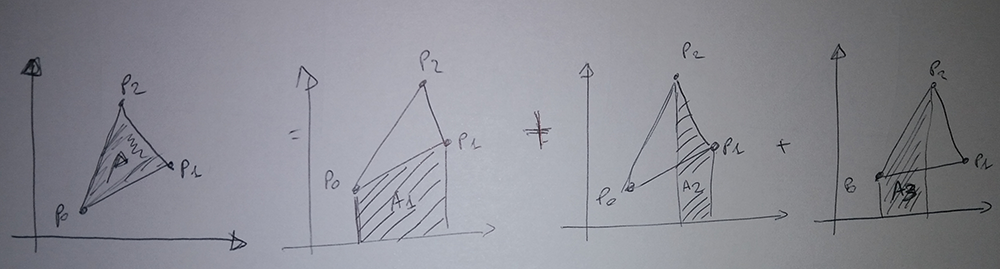
\includegraphics[width=.9\textwidth]{./notes/immagini/l28-es1.png}
\end{figure}

Se i vertici sono presi in senso antiorario l'area risulta essere positiva, perché $A_1 < 0 $ e $A_2$,$A_3 > 0$. Se invece i vertici vengono presi in senso orario, il segno delle aree cambia e quindi anche quello dell'area totale viene modificato. 

\subsection{Esercizio 3 - Calcolare l'area di un poligono}\label{esercizio-3---calcolare-larea-di-un-poligono}

Usare il risultato dell'Esercizio 1 per dimostrare per induzione su $n$ che l'area orientata di un poligono di $n$ vertici $p_0, p_1, \ldots , p_{n-1}$ che sia semplice ma non necessariamente convesso si può calcolare in tempo lineare $O(n)$ mediante la formula

$$
A = \frac{1}{2} \sum\limits_{i=1}^{n} y_i(x_{i-1} -x_{i+1})
$$

dove i vertici si intendono ordinati circolarmente in senso antiorario e quindi $x_{i-1} = x_{n-1}$ quando $i=0$ e $x_{i+1}=x_0$ quando $i=n-1$.

\subsubsection{Soluzione}

Il caso base è semplice, se $n =0$, l'area viene uguale a 0 ed è corretto, perché si tratta di un poligono degenere.

Assumendo quindi di avere l'area corretta $A_{n-1}$ per il poligono con i vertici da $p_0, \ldots p_{n-1}$, proviamo a calcolare l'area per il poligono che considera anche il vertice $p_n$.

Utilizzando la formula abbiamo che

\begin{align*}
	A_{n-1} &= \frac{1}{2} \sum\limits_{i=1}^{n-1} y_i(x_{i-1} -x_{i+1}) \\
	A_n &= \frac{1}{2} \sum\limits_{i=1}^{n} y_i(x_{i-1} -x_{i+1})  \\
			&= A_{n-1} - \underbrace{\frac{1}{2}y_0(x_{n-1} - x_1) - \frac{1}{2}y_{n-1}(x_{n-2} - x_0)}_{T_1} + \underbrace{ \frac{1}{2}y_{0}(x_{n} - x_1) + \frac{1}{2}y_{n-1}(x_{n-2} - x_n) + \frac{1}{2}y_{n}(x_{n-1} - x_0) }_{T_2} 
\end{align*}

Dove il termine $T_1$ rappresenta la porzione di $A_{n-1}$ racchiusa tra i due vertici $p_{n-1} \text{ e } p_{0}$ che prima dell'aggiunta di $p_n$ erano consecutivi, mentre il termine $T_2$ rappresenta la parte della sommatoria che cambia rispetto a quella utilizzata per calcolare $A_{n-1}$.

Raggruppando i vari termini è poi possibile riscrivere la formula come 

\begin{align*}
	A_n &= A_{n-1} + \frac{1}{2}y_{n}(x_{n-1} - x_{0}) + \frac{1}{2}y_{0}(x_{n} - x_{n-1})+ \frac{1}{2}y_{n-1}(x_{0} - x_{n})
\end{align*}

\todo{Completare}

\subsection{Esercizio 4}\label{esercizio-4}

L'angolo polare di un punto $p_i$ rispetto ad una origine $p_0$ è l'angolo formato dal vettore $\overrightarrow{p_0p_i}$ con la semiretta orizzontale destra $r$ avente origine in $p_0$.

Trovare un algoritmo che ordini un'insieme di punti per angolo polare in tempo $O(n \log n)$.

\subsubsection{Soluzione}

Se si riesce ad effettuare il confronto tra due punti per stabilire quale viene prima in tempo $O(1)$, è possibile utilizzare un qualsiasi algoritmo di ordinamento per ottenere il risultato desiderato.

Per confrontare i due punti $p_1$ e $p_2$ rispetto a $p_0$ si può calcolare $d = \textsc{Angle-Left}(p_0,p_1,p_2)$ (posizione di $p_2$ rispetto $p_1$) e le posizioni di $p_1$ e $p_2$ rispetto la semiretta $r$: $d_1 =  \textsc{Angle-Left}(p_0,r,p_1)$ e $d_2 =  \textsc{Angle-Left}(p_0,r,p_2)$.

\begin{itemize}
	\item Se $d_1 = d_2 = 0$ i due punti si trovano sulla retta $r$:
	\begin{itemize}
		\item Se solo uno dei due si trova a destra di $p_0$, viene prima quello a destra.
		\item Se tutti e due si trovano dalla stessa parte rispetto $p_0$ viene prima quello più vicino.
	\end{itemize}
	Il confronto della distanza può essere fatto considerando il valore assoluto. I prossimi casi assumono che questo non sia vero.
	\item Se i due punti stanno entrambi nel semi-piano, ovvero $d_1$ e $d_2 \geq 0$ oppure $d_1$ e $d_2 \leq 0$, resta da valutare la posizione tra i due punti:
	\begin{itemize}
		\item Se $d >0 $, $p_2$ si trova a sinistra di $p_1$ e quindi viene prima $p_1$ di $p_2$.
		\item Se $d = 0$, i due punti sono sulla stessa retta e quindi viene prima quello più vicino a $p_0$. Questo è corretto anche se uno dei due segmenti è degenere, perché vuol dire che uno dei due punti coincide con $p_0$.
		\item Se $d < 0$, $p_2$ si trova a destra di $p_1$ e quindi viene prima $p_2$ di $p_1$.
	\end{itemize}
	\item Se $d_1$ e $d_2$ sono di segno opposto viene prima il punto che si trova nel semi-piano sinistro, ovvero quello con $d_i > 0$. 
\end{itemize}

Il test può essere quindi fatto in tempo costante perché utilizza solo confronti e \textsc{Angle-Left}, quindi l'ordinamento può essere fatto in $O(n \log n)$.

\subsection{Esercizio 5}\label{esercizio-5}

Usare il risultato dell'esercizio precedente per decidere in tempo $O(n^2 \log n)$ se un insieme di $n$ punti contiene almeno 3 punti collineari.

\subsubsection{Soluzione}

Quando nell'ordinamento viene trovato $d = 0$ si ha che i punti $p_0, p_1, p_2$ sono collineari. Quindi fissato un punto si può trovare in $O(n \log n)$ se ci sono altri due punti collineari nell'insieme di punti.

Ripetendo questo procedimento cambiando ogni volta il punto di riferimento si riesce a rispondere in $O(n^2 \log n)$ alla domanda.

\subsection{Esercizio 6}\label{esercizio-6}

Un poligono è rappresentato da una sequenza di punti presi in senso antiorario che definiscono il perimetro. I lati sono i segmenti tra i due punti consecutivi. Un poligono viene detto \textbf{semplice} se i suoi lati non si intersecano.
In un poligono semplice è possibile dividere i punti in interni, esterni o di frontiera.

Un poligono semplice viene detto \textbf{convesso} se comunque presi due punti, interni o di frontiera, anche tutti gli altri punti del segmento che li unisce sono interni o di frontiera.

Trovare un algoritmo che determini se una sequenza di $n$ punti rappresenta un poligono semplice e convesso in tempo $O(n)$. Dimostrare che non è sufficiente percorrere il perimetro controllando di non svoltare mai a destra.

\subsubsection{Soluzione}

Non è sufficiente controllare solo il perimetro perché se il poligono è fatto come il logo di Airbnb, tutti i lati svoltano a sinistra, ma si intrecciano comunque tra loro.

L'idea è quindi quella di controllare se tra due lati consecutivi si svolta sempre a sinistra e se il punto di partenza del poligono si trova sempre a sinistra dell'ultimo lato del poligono considerato. Questo perché se vengono fatte troppe svolte a sinistra, prima o poi il perimetro del poligono si avvolgerà su se stesso, facendo si che il punto di partenza si trovi alla destra di almeno un lato di esso.

Si tratta quindi di controllare se la svolta è a sinistra per ogni coppia di lati consecutivi e questo può essere fatto in $O(n)$ e di controllare che per ogni lato il punto di partenza sia sempre a sinistra, fattibile anche questo in $O(n)$.
Si ottiene quindi una complessità totale di $O(n)$.

La soluzione del prof è leggermente diversa, oltre al controllo sui lati consecutivi, vengono controllati anche che \textsc{Angle-Left}$(p_0, p_{i-1}, p_i) \geq 0$ e che tutti i punti del poligono siano dalla stessa parte rispetto $\overline{p_0p_1}$, ovvero \textsc{Angle-Left}$(p_0, p_{1}, p_i) \geq 0$.

\subsection{Esercizio 7}\label{esercizio-7}

Dato un punto $P$ ed un segmento $\overline{p_1p_2}$ spiegare come si possa determinare in tempo costante $O(1)$ se il segmento interseca la semiretta orizzontale destra con origine nel punto $p$.

\subsubsection{Soluzione}

\`{E} possibile definire il punto $q$ tale che $q.y = p.y$ e $q.x = \max (p_1.x, p_2.x)$ per poi utilizzare \textsc{Segment-Intersect} tra $\overline{pq}$ e $\overline{p_1p_2}$ per determinare in tempo costante se i due segmenti si intersecano.

\subsection{Esercizio 8}\label{esercizio-8}

Usare il risultato dell'esercizio precedente per trovare un algoritmo che decide in tempo $O(n)$ se un punto $p$ è interno ad un poligono con $n$ vertici che sia semplice ma non necessariamente convesso.

\subsubsection{Soluzione}

L'idea è quella di considerare la semiretta destra che ha origine in $p$.

Se il punto $p$ è interno al poligono, la semiretta si intersecherà con un numero dispari di lati perché deve limitarsi ad ``uscire'' dal poligono, mentre se il punto è esterno la semiretta può non intersecare mai il poligono, oppure attraversarlo, intersecando un numero pari di lati. Questo è tendenzialmente vero, tranne in alcuni casi particolari, quando la semiretta interseca uno o più vertici del poligono e quando uno o più lati del poligono sono contenuto nella semiretta.

Per gestire i casi particolari occorre considerare anche il numero di vertici del poligono che hanno la stessa altezza del punto di interesse e quanti lati orizzontali del poligono sono contenuti/intersecati dalla semiretta destra.
In base a questi valori è necessario aggiustare il il contatore delle intersezioni, perché ad esempio, se c'è un lato del poligono che è contenuto nella semiretta, l'algoritmo conta 3 intersezioni, sfasando i conti.

\textbf{Quello che segue non è del tutto corretto.}

L'idea è quindi quella di controllare il numero \textit{z} di lati orizzontali contenuti nella semiretta destra  ($O(n)$) e che hanno almeno uno degli estremi a destra di \textit{p}.

Si può quindi calcolare il numero di intersezioni \textit{int} e poi aggiustarlo opportunamente prendendo in considerazione i casi particolari:

\begin{itemize}
	\item Se $z=0$, nessun lato del poligono è contenuto nella semiretta destra, il numero di intersezioni non deve essere modificato in quanto se la semiretta passa esattamente per un vertice del poligono, questa interseca due lati e quindi non altera i conti.
	\item Se $z > 0$, controllo se \textit{p} appartiene ad uno dei lati.
		\begin{itemize}
			\item Se $p$ è contenuto in un lato, allora è anche interno al poligono (tecnicamente è di frontiera)
			\item Se $p$ non è contenuto in un lato, allora il numero di intersezioni deve essere ridotto di $2z$, perché per ogni lato contenuto nella semiretta, vengono intersecati 3 lati del poligono:
			$$
			int = int - 2z
			$$
		\end{itemize}
\end{itemize}

Se alla fine degli aggiustamenti il numero di intersezioni è pari, allora \textit{p} è un punto esterno, in caso contrario è un punto interno.

Per quanto riguarda la complessità, c'è un $O(n)$ per il calcolo di $z$, un $O(n)$ per il calcolo delle intersezioni e un $O(z)$ per il controllo se il punto $p$ è all'interno di uno dei lati che interseca la semiretta. Dal momento che $z$ è sicuramente $<n$ e che tutte queste complessità si sommano, l'algoritmo risponde in tempo $O(n)$. 
 